\title{Aula 12 - IPsec}

\author{Prof. Gabriel Rodrigues Caldas de Aquino}

\institute
{
    Instituto de Computação \\
    Universidade Federal do Rio de Janeiro\\
    gabrielaquino@ic.ufrj.br% Your institution for the title page
}
\date{Compilado em: \\ \today} % Date, can be changed to a custom date

%----------------------------------------------------------------------------------------
%    PRESENTATION SLIDE
%----------------------------------------------------------------------------------------



\begin{frame}
    % Print the title page as the first slide
    \titlepage
\end{frame}

\begin{frame}{IPsec: O Protocolo IP de Segurança}
    \begin{itemize}
        \item Provê segurança na camada de rede.
        \item Protege datagramas IP entre quaisquer entidades (dispositivos finais (\textit{hosts}), roteadores).
        \item Usado para criar Redes Privadas Virtuais (VPNs) sobre a Internet pública.
        \item Definido pelo IAB como essencial para o IPv6 (autenticação e criptografia).
        \item Projetado para ser compatível tanto com IPv4 quanto com IPv6.
        \item Atualmente, muitos fabricantes já oferecem suporte ao IPsec.
    \end{itemize}
\end{frame}

\begin{frame}{Relembrando encapsulamento em redes}


    \begin{figure}
        \centering
        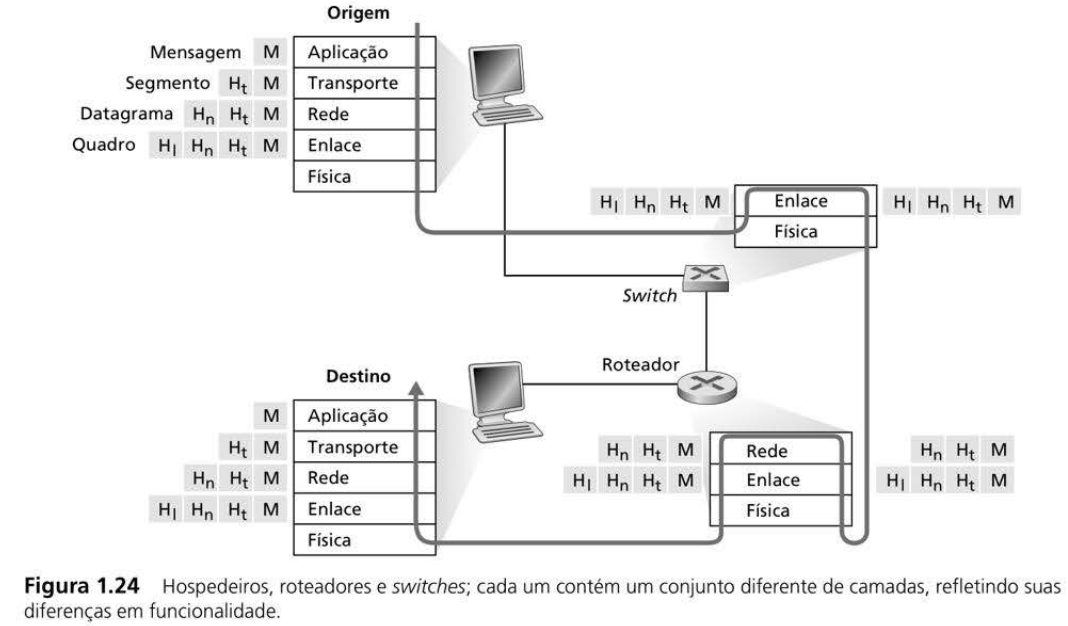
\includegraphics[width=0.7\textwidth]{Figuras/encapsulamento-pilha-protocolos.png}
    \end{figure}



\end{frame}

\begin{frame}{Relembrando o formato do datagrama IPv4}


    \begin{figure}
        \centering
        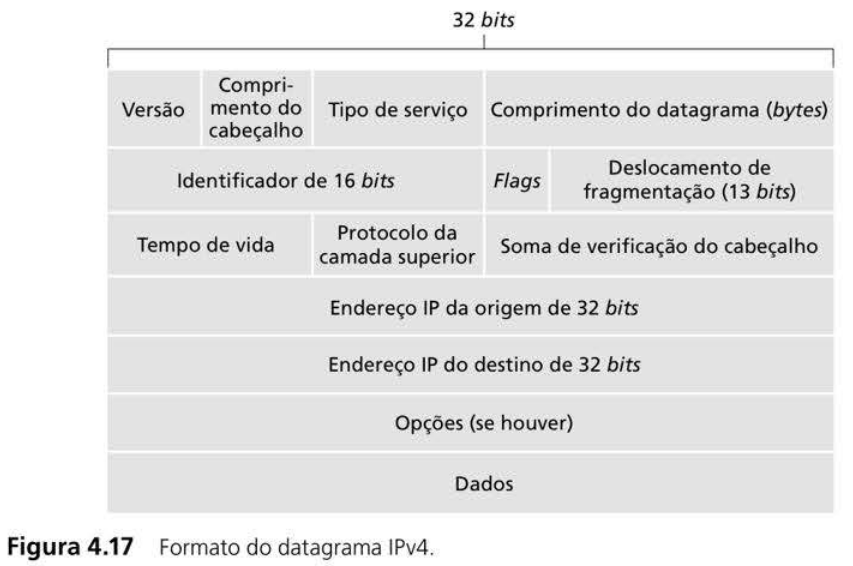
\includegraphics[width=0.7\textwidth]{Figuras/formato-datagrama-ipv4.png}
    \end{figure}



\end{frame}

\begin{frame}{Áreas Funcionais da Segurança em Nível IP}
    \begin{itemize}
        \item A segurança em nível IP abrange três áreas funcionais:
    \end{itemize}

    \begin{block}{1. Autenticação}
        \begin{itemize}
            \item Garante que o pacote foi realmente enviado pela fonte identificada.
            \item Assegura que o pacote não foi alterado durante o trânsito.
        \end{itemize}
    \end{block}

    \begin{block}{2. Confidencialidade}
        \begin{itemize}
            \item Permite aos nós da rede cifrar (criptografar) mensagens.
            \item Previne a espionagem (eavesdropping) por terceiros.
        \end{itemize}
    \end{block}

    \begin{block}{3. Gerenciamento de Chaves}
        \begin{itemize}
            \item Trata da troca segura de chaves entre as partes.
        \end{itemize}
    \end{block}
\end{frame}

\begin{frame}{O Conceito de Sigilo na Camada de Rede}
    \begin{itemize}
        \item O que significa prover sigilo na camada de rede?
              \begin{itemize}
                  \item A entidade remetente (hospedeiro ou roteador) cifra as \textbf{cargas úteis (payloads)} de todos os datagramas que envia.
              \end{itemize}

        \item O que é a carga útil (payload)?
              \begin{itemize}
                  \item Segmento TCP
                  \item Segmento UDP
                  \item Mensagem ICMP
                  \item Mensagem SNMP, etc.
              \end{itemize}

        \item Resultado: \textbf{"Cobertura Total" }
              \begin{itemize}
                  \item Todos os dados (e-mails, páginas Web, mensagens de gerenciamento) ficam ocultos de intrusos.
              \end{itemize}
    \end{itemize}
\end{frame}



\begin{frame}{Outros Serviços de Segurança da Camada de Rede}
    Além da confidencialidade, um protocolo de segurança da camada de rede pode prover:
    \begin{itemize}

        \item \textbf{Autenticação da Origem}
              \begin{itemize}
                  \item Permite à entidade destinatária verificar a origem (remetente) do datagrama protegido.
              \end{itemize}

        \item \textbf{Integridade dos Dados}
              \begin{itemize}
                  \item Permite à entidade destinatária verificar se o datagrama sofreu qualquer adulteração durante o trânsito.
              \end{itemize}

        \item \textbf{Prevenção do Ataque de Repetição (Replay Attack)}
              \begin{itemize}
                  \item Permite ao destinatário (Bob) detectar quaisquer datagramas duplicados que um atacante possa inserir no fluxo.
              \end{itemize}
        \item \textbf{Característica:} IPsec pode \textbf{criptografar e/ou autenticar todo o tráfego no nível IP}.
    \end{itemize}


\end{frame}
\begin{frame}{Aplicações Comuns do IPsec}

    \begin{itemize}
        \item O IPsec pode ser usado em LANs, WANs (públicas/privadas) e na Internet.
        \item Todas as aplicações distribuídas se beneficiam, sem necessidade de modificação.

        \item \textbf{Exemplos de uso:}
              \begin{itemize}
                  \item \textbf{Conectividade Segura de Filiais (VPN):}
                        \begin{itemize}
                            \item Permite construir uma VPN segura sobre a Internet.
                            \item Reduz custos e a necessidade de redes privadas.
                        \end{itemize}

                  \item \textbf{Acesso Remoto Seguro:}
                        \begin{itemize}
                            \item Usuários remotos (viajantes, telecommuters) acessam a rede da empresa de forma segura através de um ISP local.
                        \end{itemize}

                  \item \textbf{Conectividade Extranet/Intranet com Parceiros:}
                        \begin{itemize}
                            \item Protege a comunicação com outras organizações (autenticação, confidencialidade, troca de chaves).
                        \end{itemize}

                  \item \textbf{Reforço à Segurança de E-commerce:}
                        \begin{itemize}
                            \item Adiciona segurança, mesmo que as aplicações Web já possuam protocolos de segurança próprios.
                        \end{itemize}
              \end{itemize}
    \end{itemize}
\end{frame}

\begin{frame}{Benefícios do IPsec}
    \begin{itemize}
        \item \textbf{Implementação em Firewall/Roteador}
              \begin{itemize}
                  \item Aplica segurança forte a todo o tráfego que cruza o perímetro.
                  \item O tráfego interno (workgroup) não sofre overhead de processamento.
              \end{itemize}

        \item \textbf{Resistência a Bypass}
              \begin{itemize}
                  \item Difícil de contornar (bypass) se o firewall IPsec for a única entrada da Internet.
              \end{itemize}

        \item \textbf{Transparência para Aplicações}
              \begin{itemize}
                  \item Atua abaixo da camada de transporte (TCP/UDP).
                  \item Não exige mudança de software em usuários ou servidores.
                  \item Aplicações de camada superior não são afetadas.
              \end{itemize}
        \item \textbf{Transparência para o Usuário Final}
              \begin{itemize}
                  \item Não é necessário treinar os usuários sobre os mecanismos de segurança.
                  \item Não é preciso gerenciar chaves por usuário (emitir/revogar).
              \end{itemize}

        \item \textbf{Flexibilidade (Segurança Individual)}
              \begin{itemize}
                  \item Pode prover segurança para usuários individuais, se necessário.
                  \item Útil para trabalhadores remotos (off-site).
                  \item Permite criar sub-redes virtuais seguras para aplicações sensíveis.
              \end{itemize}
    \end{itemize}
\end{frame}

\begin{frame}{IPsec e Redes Privadas Virtuais (VPNs)}
    \begin{itemize}
        \item \textbf{O Cenário:}
              \begin{itemize}
                  \item Instituições que se estendem por diversas regiões geográficas.
              \end{itemize}

        \item \textbf{A Necessidade:}
              \begin{itemize}
                  \item Desejam ter sua própria rede IP.
                  \item Objetivo: Permitir que seus hospedeiros e servidores enviem dados uns aos outros de forma segura e sigilosa.
              \end{itemize}

        \item \textbf{A Solução Tradicional: Rede Privada}
              \begin{itemize}
                  \item Definição: Uma rede física independente, reservada a uma instituição particular.
                  \item Características:
                  \item É completamente separada da Internet pública.
                  \item Requer infraestrutura própria: roteadores, enlaces e DNS.
              \end{itemize}

        \item \textbf{O Problema da Rede Privada:}
              \begin{itemize}
                  \item Custo muito elevado.
                  \item A instituição precisa comprar, instalar e manter sua própria infraestrutura de rede física.
              \end{itemize}
    \end{itemize}
\end{frame}

\begin{frame}{A Solução: Rede Privada Virtual (VPN)}
    \begin{itemize}
        \item  VPNs operam "em cima" (sobre) da Internet pública.
        \item O tráfego é  \textbf{criptografado} e enviado através da infraestrutura da Internet pública.
        \item Não é necessária uma rede fisicamente independente e dedicada.

        \item A criptografia é aplicada \textbf{antes} que os pacotes entrem na Internet pública.
    \end{itemize}


    % Você pode inserir sua figura aqui
    \begin{figure}
        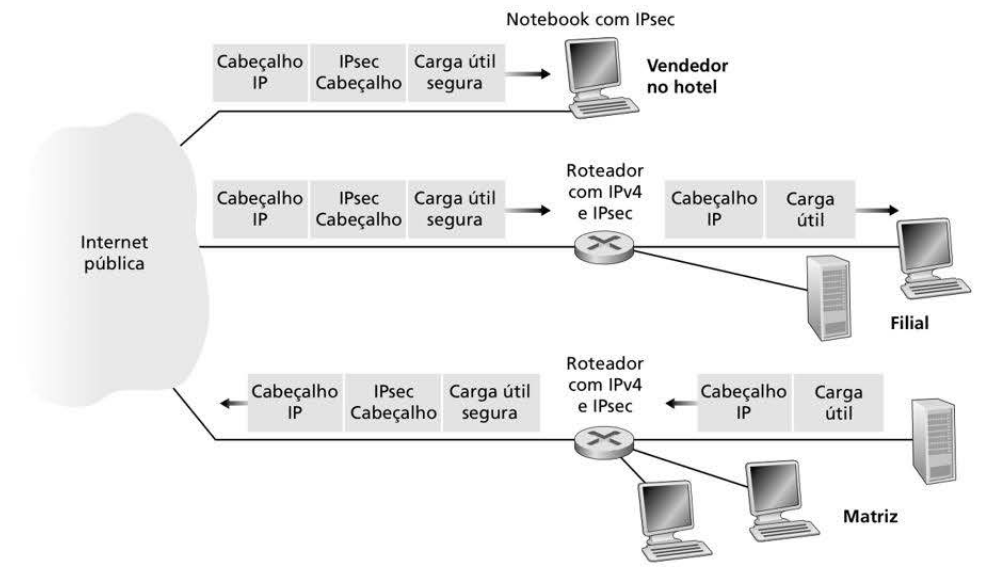
\includegraphics[width=0.68\textwidth]{Figuras/ipsec-vpn.png}
        \label{fig:vpn}
    \end{figure}
\end{frame}

\begin{frame}{VPN: Cenário de Exemplo e Fluxo de Tráfego}
    \begin{itemize}
        \item \textbf{Componentes da Instituição (Exemplo):}
              \begin{itemize}
                  \item Matriz, Filial e outros acessando da Internet

              \end{itemize}

        \item \textbf{Fluxo 1: Comunicação Interna (Dentro de um Local)}
              \begin{itemize}
                  \item Ex: Hospedeiro na Matriz $\leftrightarrow$ Hospedeiro na Matriz.
                  \item Ex: Hospedeiro na Filial $\leftrightarrow$ Hospedeiro na Filial.
                  \item Método: IP v4 padrão (sem IPsec). O tráfego não sai para a rede pública.
              \end{itemize}

        \item \textbf{Fluxo 2: Comunicação Externa (Entre Locais via VPN)}
              \begin{itemize}
                  \item Ex: Hospedeiro na Matriz $\leftrightarrow$ Hospedeiro na Filial.
                  \item Ex: Vendedor Viajante $\leftrightarrow$ Hospedeiro na Matriz.
                  \item Caminho: O tráfego deve cruzar a Internet pública.
                  \item Método: O tráfego é \textbf{codificado (criptografado)} antes de entrar na Internet (usando IPsec).
              \end{itemize}
    \end{itemize}
\end{frame}

\begin{frame}{Tráfego Misto: IPsec e IPv4 Comum}
    \begin{itemize}
        \item \textbf{Ponto Importante:}
              \begin{itemize}
                  \item Nem todo o tráfego enviado à Internet pelos roteadores de borda ou pelos notebooks será protegido por IPsec.
              \end{itemize}

        \item \textbf{Exemplo: Acesso à Internet Pública}
              \begin{itemize}
                  \item Um hospedeiro na matriz quer acessar um servidor Web comum (ex: Amazon, Google).
                  \item Este tráfego não é destinado à VPN.
              \end{itemize}

        \item \textbf{Resultado: Coexistência de Tráfego}
              \begin{itemize}
                  \item O roteador de borda (e os notebooks) emitirão \textbf{ambos} os tipos de datagramas para a Internet:
                        \begin{itemize}
                            \item Datagramas IPv4 comuns (para tráfego público).
                            \item Datagramas IPsec seguros (para tráfego da VPN).
                        \end{itemize}
              \end{itemize}
    \end{itemize}
\end{frame}

\begin{frame}{VPN: Fluxo de Tráfego (Matriz $\rightarrow$ Vendedor Viajante)}
    \begin{itemize}
        \item \textbf{1. Na Matriz (Origem)}
              \begin{itemize}
                  \item Um hospedeiro envia um datagrama IPv4 padrão (ex: TCP/UDP).
              \end{itemize}

        \item \textbf{2. No Roteador de Borda (Gateway IPsec da Matriz)}
              \begin{itemize}
                  \item Intercepta o datagrama IPv4.
                  \item Converte o datagrama IPv4 em um datagrama \textbf{IPsec}.
                  \item Encaminha o pacote IPsec para a Internet.
              \end{itemize}

        \item \textbf{3. Na Internet (Trânsito)}
              \begin{itemize}
                  \item O datagrama IPsec possui um cabeçalho IPv4 tradicional (externo).
                  \item Roteadores da Internet o processam como um datagrama IPv4 comum.
              \end{itemize}

        \item \textbf{4. Estrutura do Pacote IPsec (no Trânsito)}
              \begin{itemize}
                  \item A carga útil (payload) do datagrama IPsec contém:
                        \begin{itemize}
                            \item Um \textbf{cabeçalho IPsec} (para processamento de segurança).
                            \item A carga útil original (ex: segmento TCP/UDP), que está \textbf{codificada} (criptografada).
                        \end{itemize}
              \end{itemize}

        \item \textbf{5. No Notebook do Vendedor (Destino)}
              \begin{itemize}
                  \item O S.O. recebe o datagrama IPsec.
                  \item \textbf{Decodifica} a carga útil (descriptografa).
                  \item Verifica outros serviços (ex: integridade dos dados).
                  \item Passa a carga útil original (não codificada) para a camada superior (TCP ou UDP).
              \end{itemize}
    \end{itemize}
\end{frame}

\begin{frame}{Protocolos Principais do IPsec: AH vs. ESP}
    O conjunto IPsec possui dois protocolos principais para envio de dados seguros (entre hospedeiros ou roteadores):
    \begin{itemize}


        \item \textbf{1. Protocolo Cabeçalho de Autenticação (AH - Authentication Header)}
              \begin{itemize}


                  \item \textbf{Provê} Autenticação da Origem.
                  \item \textbf{Provê} Integridade dos Dados.

                  \item \textbf{NÃO} provê Sigilo (Confidencialidade).
              \end{itemize}

        \item \textbf{2. Protocolo Carga de Segurança de Encapsulamento (ESP - Encapsulating Security Payload)}
              \begin{itemize}


                  \item \textbf{Provê} Autenticação da Origem.
                  \item \textbf{Provê} Integridade dos Dados.
                  \item \textbf{Provê} \textbf{Sigilo (Confidencialidade)} $\leftarrow$ (Função combinada de autenticação/criptografia).

              \end{itemize}
    \end{itemize}
\end{frame}

\begin{frame}{O Foco no ESP (AH é Deprecated)}
    \begin{itemize}
        \item \textbf{Por que o ESP é muito mais utilizado?}
              \begin{itemize}
                  \item O Sigilo (Criptografia) é muitas vezes essencial para VPNs.
                  \item VPNs geralmente desejam \textbf{autenticação E criptografia} para:
                        \begin{itemize}
                            \item 1. Impedir que usuários não autorizados penetrem na rede.
                            \item 2. Impedir que espiões (eavesdroppers) na Internet leiam as mensagens.
                        \end{itemize}
              \end{itemize}

        \item \textbf{O Status Atual do AH}: é \textbf{deprecated} (obsoleto)
              \begin{itemize}

                  \item Motivo: O próprio protocolo ESP já fornece a autenticação da mensagem.
                  \item O AH é mantido no IPsecv3 apenas para \textit{backward compatibility} (compatibilidade retroativa).
                  \item \textbf{Não deve ser usado em novas aplicações.}
              \end{itemize}

        \item \textbf{Foco atual:} \textbf{ESP}.

    \end{itemize}
\end{frame}

\begin{frame}{Associações de Segurança (SA)}
    \begin{itemize}
        \item Datagramas IPsec são enviados entre pares de entidades da rede (hospedeiro $\leftrightarrow$ hospedeiro, roteador $\leftrightarrow$ roteador, etc.).

        \item \textbf{O que é uma Associação de Segurança (SA - \textit{Security Association})?}
              \begin{itemize}

                  \item É uma \textbf{conexão lógica} da camada de rede.
                  \item Criada \textbf{antes} que a entidade remetente possa enviar datagramas IPsec à entidade destinatária.
              \end{itemize}

        \item \textbf{Característica Chave: Unidirecional}
              \begin{itemize}
                  \item Uma SA é uma conexão lógica \textbf{simples} (simplex).
                  \item Ela flui em apenas uma direção: do remetente para o destinatário.
              \end{itemize}

        \item \textbf{Comunicação Bidirecional (Mútua)}
              \begin{itemize}
                  \item Se duas entidades querem enviar dados seguros entre si (nos dois sentidos): Precisam ser estabelecidas \textbf{duas SAs} (duas conexões lógicas).
                  \item Uma SA em cada direção.
              \end{itemize}
    \end{itemize}
\end{frame}

\begin{frame}{Exemplo: Contagem de SAs em uma VPN}
    \begin{itemize}
        \item \textbf{Cenário (Instituição):}
              \begin{itemize}
                  \item 1 Matriz.
                  \item 1 Filial.
                  \item $n$ Vendedores Viajantes (notebooks).
              \end{itemize}

        \item \textbf{Fluxos de Tráfego IPsec (Bidirecional):}
              \begin{itemize}
                  \item Tráfego bidirecional entre o roteador de borda da Matriz e o roteador de borda da Filial.
                  \item Tráfego bidirecional entre o roteador de borda da Matriz e CADA UM dos $n$ Vendedores.
              \end{itemize}

        \item \textbf{Cálculo - Quantidade de SA:}
              \begin{itemize}
                  \item \textbf{Matriz $\leftrightarrow$ Filial:}
                        \begin{itemize}
                            \item 1 SA (Matriz $\rightarrow$ Filial)
                            \item 1 SA (Filial $\rightarrow$ Matriz)
                            \item \textit{Subtotal = 2 SAs}
                        \end{itemize}
                  \item \textbf{Matriz $\leftrightarrow$ $n$ Vendedores:}
                        \begin{itemize}
                            \item Para cada vendedor, são necessárias 2 SAs (uma em cada direção).
                            \item \textit{Subtotal = 2 $\times$ n SAs}
                        \end{itemize}
              \end{itemize}

        \item \textbf{Total de SAs na VPN:}
              \begin{itemize}
                  \item Total = (SAs da Filial) + (SAs dos Vendedores)
                  \item Total = 2 + 2$n$ SAs
              \end{itemize}
    \end{itemize}
\end{frame}

\begin{frame}{O Banco de Dados de Associações de Segurança (SAD)}
    \begin{itemize}
        \item Toda implementação IPsec inclui um \textbf{Banco de Dados de Associações de Segurança} (SAD - Security Association Database).

        \item Este banco de dados armazena e define todos os parâmetros associados a cada SA (Associação de Segurança) ativa.

        \item Uma SA é caracterizada por um conjunto de parâmetros específicos. \textbf{Que vamos ver nos próximos slides}

        \item Uma entidade IPsec (roteador ou hospedeiro) armazena informações de estado para \textbf{muitas SAs} simultaneamente.

        \item \textbf{Relembrando o Exemplo da VPN:}
              \begin{itemize}
                  \item Cenário: 1 Matriz, 1 Filial e $n$ vendedores.
                  \item O roteador de borda da Matriz guarda informações de estado para \textbf{(2 + 2$n$)} SAs.
              \end{itemize}
    \end{itemize}


\end{frame}

\begin{frame}{O SPD - Security Policy Database}
    \textbf{O Problema:} R1 recebe um datagrama IPv4 da rede interna destinado a um IP de fora.
    \begin{itemize}

        \item \textbf{Como R1 sabe }se este datagrama deve ser convertido em IPsec (ou enviado como IPv4 comum)?
              \begin{itemize}
                  \item ... e se for IPsec, qual SA (dentre as várias no SAD) ele deve usar?
              \end{itemize}
    \end{itemize}

    \begin{itemize}



        \item \textbf{A Solução: O Banco de Dados de Política de Segurança (SPD)}
              \begin{itemize}

                  \item A entidade IPsec (R1) mantém esta \textit{outra} estrutura de dados (além do SAD).
                  \item O SPD indica \textbf{quais tipos} de datagramas serão processados pelo IPsec.
                  \item A decisão é baseada em: Endereço IP remetente, Endereço IP destinatário, e Tipo do protocolo (TCP/UDP).
                  \item O SPD também aponta para qual SA deve ser usada.
              \end{itemize}

        \item \textbf{A Diferença Chave: SPD vs. SAD}
              \begin{itemize}
                  \item \textbf{SPD (Política):} Indica \textbf{"O QUE"} fazer com um datagrama (Processar com IPsec, Descartar, Deixar passar).
                  \item \textbf{SAD (Associação):} Indica \textbf{"COMO"} fazer o IPsec (Chaves de criptografia/autenticação, algoritmos, SPI, etc).
              \end{itemize}
    \end{itemize}
\end{frame}

\begin{frame}{Informações de Estado da SA (Exemplo: Roteador R1)}


    \begin{figure}
        \centering
        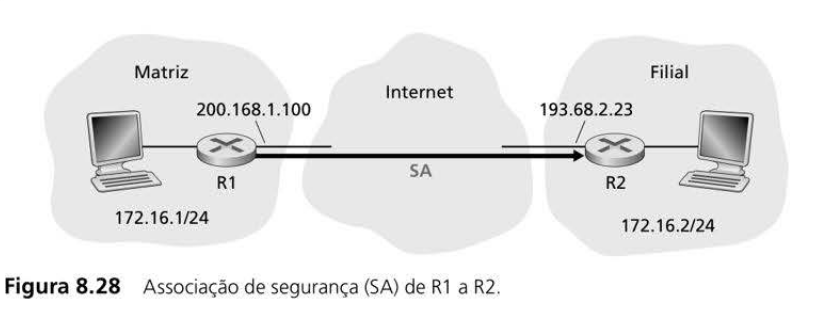
\includegraphics[width=0.7\textwidth]{Figuras/ipsec-e-SAs.png}
    \end{figure}



\end{frame}

\begin{frame}{Uso das Informações de Estado da SA (Exemplo R1 $\rightarrow$ R2)}
    \begin{itemize}
        \item \textbf{No Remetente (Roteador R1)}
              \begin{itemize}
                  \item Quando R1 precisa construir um datagrama IPsec para encaminhar por essa SA:
                  \item Ele acessa as informações de estado (SPI, chaves, algoritmos) da SA.
                  \item Usa essas informações para determinar como deve \textbf{autenticar} e \textbf{criptografar} o datagrama.
              \end{itemize}

        \item \textbf{No Destinatário (Roteador R2)}
              \begin{itemize}
                  \item R2 mantém as \textit{mesmas} informações de estado sobre essa SA (identificada pelo SPI).
                  \item Ele as usa para \textbf{autenticar} (verificar a integridade) e \textbf{decodificar} (descriptografar) qualquer datagrama IPsec que chegar da SA.
              \end{itemize}
    \end{itemize}
\end{frame}

\begin{frame}{Informações de Estado da SA (Exemplo: Roteador RI)}

    O Roteador R1 manterá as informações de estado sobre essa SA:

    \begin{itemize}
        \item Um identificador de 32 bits para a SA: \textbf{Índice de Parâmetro de Segurança (SPI)}


        \item As interfaces da SA:
              \begin{itemize}
                  \item Interface remetente (Origem): 200.168.1.100
                  \item Interface destinatária (Destino): 193.68.2.23
              \end{itemize}

        \item Parâmetros de Criptografia (para Sigilo):
              \begin{itemize}
                  \item O tipo de criptografia (ex: 3DES com CBC).
                  \item A chave de criptografia.
              \end{itemize}

        \item Parâmetros de Integridade (para Autenticação):
              \begin{itemize}
                  \item O tipo de verificação de integridade (ex: HMAC com MD5).
                  \item A chave de autenticação.
              \end{itemize}
    \end{itemize}
\end{frame}

\begin{frame}{Parâmetros da SA (Parte 1)}
    \begin{itemize}
        \item \textbf{Contador de Número de Sequência (Sequence number counter)}
              \begin{itemize}
                  \item Um valor de 32 bits usado para gerar o campo "Sequence Number" nos cabeçalhos AH ou ESP
                  \item Essencial para o antireplay.
              \end{itemize}

        \item \textbf{Estouro do Contador (Sequence counter overflow)}
              \begin{itemize}
                  \item Uma "flag" que indica se o estouro (overflow) do contador deve:
                        \begin{itemize}
                            \item Gerar um evento auditável (log).
                            \item Impedir a transmissão de mais pacotes nesta SA.
                        \end{itemize}
              \end{itemize}

        \item \textbf{Janela Antireplay (Antireplay window)}
              \begin{itemize}
                  \item Define uma "janela deslizante" (sliding window).
                  \item Usada para determinar se um pacote AH ou ESP recebido é um \textit{replay} (pacote duplicado/malicioso).
                  \item O número de sequência do pacote deve estar dentro desta janela.
              \end{itemize}
    \end{itemize}
\end{frame}

\begin{frame}{Parâmetros da SA (Parte 2)}
    \begin{itemize}

        \item \textbf{Informações ESP}
              \begin{itemize}
                  \item Algoritmo de criptografia e autenticação.
                  \item Chaves, Valores de Inicialização (IVs), tempos de vida das chaves e parâmetros relacionados ao ESP.
              \end{itemize}

        \item \textbf{Tempo de Vida da SA (Lifetime)}
              \begin{itemize}
                  \item Um intervalo de tempo ou uma contagem de bytes.
                  \item Após atingido, a SA deve ser substituída por uma nova SA (e novo SPI) ou terminada.
              \end{itemize}

        \item \textbf{Modo do Protocolo IPsec (Protocol mode)}
              \begin{itemize}
                  \item Define o modo de operação: Túnel (Tunnel) ou Transporte (Transport)
              \end{itemize}

        \item \textbf{Path MTU}
              \begin{itemize}
                  \item Armazena o "Maximum Transmission Unit" (tamanho máximo do pacote) observado no caminho.
                  \item Usado para evitar fragmentação de pacotes.
                  \item Inclui variáveis de "envelhecimento" (aging).
              \end{itemize}
    \end{itemize}
\end{frame}

\begin{frame}{O Datagrama IPsec: Modo Túnel vs. Modo Transporte}
    \begin{itemize}
        \item Analisando o datagrama IPsec.

        \item O IPsec possui \textbf{duas formas diferentes de pacotes} (dois modos de operação):
              \begin{itemize}
                  \item \textbf{Modo Túnel (Tunnel Mode)}
                  \item \textbf{Modo Transporte (Transport Mode)}
              \end{itemize}

        \item \textbf{Comparação de Uso:}
              \begin{itemize}
                  \item O \textbf{Modo Túnel} é o mais apropriado para o cenário de VPNs (que vimos anteriormente).
                  \item Por esta razão, o Modo Túnel é \textbf{mais implementado} do que o Modo Transporte.
              \end{itemize}

        \item \textbf{Foco da Aula:}
              \begin{itemize}
                  \item A partir de agora vamos nos concentrar \textbf{exclusivamente no Modo Túnel}.
                  \item (Uma vez que se tem uma compreensão sólida do Modo Túnel, é fácil aprender o Modo Transporte).
              \end{itemize}
    \end{itemize}
\end{frame}
\begin{frame}{Processo de Criação do Datagrama ESP (Modo Túnel)  - Parte 1}
    O processo de encapsulamento (ex: no roteador de borda) segue estes passos
    \begin{itemize}


        \item \textbf{1. Criptografia e criação da mensagem}
              \begin{itemize}
                  \item Pega-se o datagrama IP original (que será protegido).
                  \item Criptografa-se este datagrama (ele se torna o campo "Payload Data").
                  \item Anexa-se na frente dele o "Cabeçalho ESP" (SPI + Seq. Number).
                  \item O pacote resultante é o Cabeçalho ESP + Carga Criptografada + Trailers ESP.
              \end{itemize}

        \item \textbf{2. Autenticação (MAC/ICV)}
              \begin{itemize}
                  \item Cria-se uma autenticação MAC (ou ICV - Integrity Check Value) sobre o datagrama inteiro.
                  \item Utiliza-se o algoritmo (ex: HMAC) e a chave de autenticação especificados na SA.
              \end{itemize}
    \end{itemize}
\end{frame}
\begin{frame}{Processo de Criação do Datagrama ESP (Modo Túnel) - Parte 2}
    \begin{itemize}

        \item \textbf{3. Formação da Carga Útil (Payload) ESP}
              \begin{itemize}
                  \item Anexa-se o MAC (ICV) atrás do datagrama.
                  \item O resultado (Cabeçalho ESP + Carga Criptografada + Trailers + MAC) forma a \textbf{Carga Útil ESP} completa.
              \end{itemize}

        \item \textbf{4. Criação do Novo Cabeçalho IP (Modo Túnel)}
              \begin{itemize}
                  \item Por fim, cria-se um \textbf{novo cabeçalho IP} (IPv4 clássico, 20 bytes).
                  \item Este novo cabeçalho é anexado \textbf{antes} da Carga Útil ESP.
                  \item Este é o cabeçalho que os roteadores da Internet irão ler.
              \end{itemize}
    \end{itemize}
\end{frame}

\begin{frame}{Datagrama IPSec}


    \begin{figure}
        \centering
        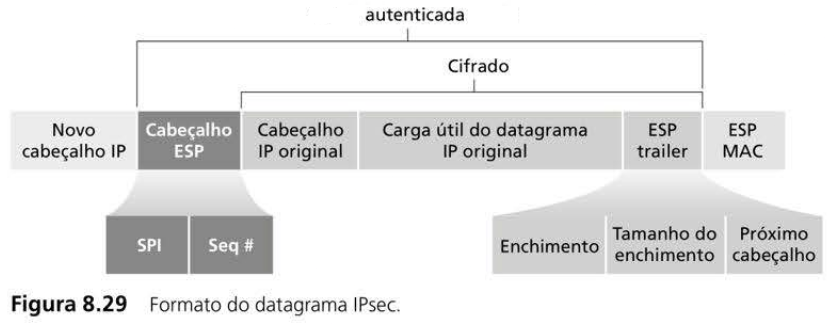
\includegraphics[width=0.9\textwidth]{Figuras/datagrama-ipsec.png}


    \end{figure}



\end{frame}



\begin{frame}{O Datagrama IPsec Resultante (Modo Túnel)}
    \begin{itemize}


        \item \textbf{A Carga Útil (Payload) deste datagrama contém:}
              \begin{itemize}
                  \item O Cabeçalho ESP (SPI, Seq. Number).
                  \item O \textbf{Datagrama IP Original} (cifrado).
                  \item O Trailer ESP (Padding, Pad Length, Next Header) (cifrado).
                  \item O Campo de Autenticação ESP (ICV/MAC).
              \end{itemize}

        \item \textbf{Cabeçalho IP Original (Interno e Cifrado)}
              \begin{itemize}
                  \item Contém os endereços dos \textit{hospedeiros finais}.
                  \item Endereço IP Remetente (Ex): \texttt{172.16.1.17}
                  \item Endereço IP Destinatário (Ex): \texttt{172.16.2.48}
                  \item Estes endereços são \textbf{cifrados} e invisíveis para a Internet.
              \end{itemize}

        \item \textbf{Novo Cabeçalho IP (Externo e Visível)}
              \begin{itemize}
                  \item Contém os endereços das \textit{extremidades do túnel} (os gateways IPsec).
                  \item Endereço IP Remetente (Ex): \texttt{200.168.1.100}
                  \item Endereço IP Destinatário (Ex): \texttt{193.68.2.23}
                  \item O campo "Protocolo" deste novo cabeçalho é \textbf{50} (indicando ESP), e não TCP(6) ou UDP(17).
              \end{itemize}
    \end{itemize}
\end{frame}

\begin{frame}{Revisão: O Cabeçalho ESP (Enviado em Aberto)}
    \begin{itemize}
        \item O "Cabeçalho ESP" é anexado na frente da unidade cifrada (payload + trailer).
        \item Este cabeçalho \textbf{não é criptografado} (é enviado "em aberto" / "clear text").
        \item Ele consiste em dois campos principais:

        \item \textbf{1. O Índice de Parâmetro de Segurança (SPI)}
              \begin{itemize}
                  \item \textbf{Função:} Indica à entidade destinatária (ex: R2) a qual Associação de Segurança (SA) este datagrama pertence.
                  \item \textbf{Ação no Destino:} A entidade usa o SPI para indexar (localizar) rapidamente a SA correta em seu Banco de Dados (SAD).
                  \item Ao localizar a SA, o destino sabe quais algoritmos e chaves deve usar para autenticar e decriptar o pacote.
              \end{itemize}

        \item \textbf{2. O Campo de Número de Sequência}
              \begin{itemize}
                  \item \textbf{Função:} É usado para a proteção contra ataques de repetição (replay attacks).
                  \item (O destinatário verifica este número contra a sua "janela antireplay" definida na SA).
              \end{itemize}
    \end{itemize}
\end{frame}

\begin{frame}{O Trailer ESP: Campos e Criptografia}
    \begin{itemize}
        \item O trailer ESP consiste em três campos:
        \item \textbf{Importante:} O trailer é adicionado ao datagrama IP original \textbf{antes} da cifragem.

        \item \textbf{1. Enchimento (Padding)}
              \begin{itemize}
                  \item \textbf{O quê:} Bytes sem significado.
                  \item \textbf{Por quê:} Cifras de bloco exigem que a mensagem a ser cifrada seja um múltiplo inteiro do comprimento de bloco (ex: 128 bits para o AES).
                  \item O enchimento é usado para "completar" o bloco.
              \end{itemize}

        \item \textbf{2. Tamanho do Enchimento (Pad Length)}
              \begin{itemize}
                  \item \textbf{O quê:} Um campo que indica quantos bytes de enchimento (\textit{padding}) foram inseridos.
                  \item \textbf{Por quê:} Permite à entidade destinatária saber exatamente quanto enchimento deve remover após a decriptação.
              \end{itemize}

        \item \textbf{3. Próximo Cabeçalho (Next Header)}
              \begin{itemize}
                  \item \textbf{O quê:} Identifica o tipo de dados da carga útil (o datagrama original).
                  \item \textbf{Por quê:} Informa ao S.O. do destinatário para qual protocolo entregar o pacote decriptado (ex: TCP, UDP, ICMP).
              \end{itemize}

        \item \textbf{Resumo do Processo de Cifragem:}
              \begin{itemize}
                  \item Os [Dados da Carga Útil (Datagrama IP original)] e o [Trailer ESP] são concatenados.
                  \item O resultado concatenado é então \textbf{cifrado} como uma única unidade.
              \end{itemize}
    \end{itemize}
\end{frame}

\begin{frame}{O MAC de Autenticação ESP (ICV)}
    \begin{itemize}
        \item Além da criptografia, a entidade remetente anexa uma \textbf{Autenticação MAC} (MAC - Message Authentication Code) ou ICV.

        \item \textbf{Sobre o que o MAC é calculado?}
              \begin{itemize}
                  \item O remetente calcula o MAC sobre \textbf{toda o datagrama}.
              \end{itemize}

        \item \textbf{O que  o cálculo do MAC?}
              \begin{itemize}
                  \item O Cabeçalho ESP (SPI + Seq. Number) - (em aberto).
                  \item O Datagrama IP original (já criptografado).
                  \item O Trailer ESP (Padding, etc.) (já criptografado).
              \end{itemize}

        \item \textbf{Como o MAC é calculado? (Revisão)}
              \begin{itemize}
                  \item O remetente anexa uma \textbf{chave MAC secreta} definida na SA.
                  \item Em seguida, calcula um \textbf{hash de tamanho fixo} do resultado (ex: HMAC-MD5 ou HMAC-SHA1).
                  \item Este hash é o MAC/ICV, que é anexado ao final do pacote.
              \end{itemize}
    \end{itemize}
\end{frame}

\begin{frame}{Processamento no Destino (Exemplo: Roteador R2)}
    \begin{itemize}
        \item Quando R2 recebe o datagrama IPsec (destino: R2, protocolo: 50):

        \item \textbf{1. Identificação da SA:}
              \begin{itemize}
                  \item R2 entende que é um pacote ESP (Protocolo 50).
                  \item Ele lê o campo \textbf{SPI} (no cabeçalho ESP) para determinar a qual SA o datagrama pertence (procurando no SAD).
              \end{itemize}

        \item \textbf{2. Verificação de Autenticidade/Integridade:}
              \begin{itemize}
                  \item R2 calcula o MAC sobre o datagrama (usando a chave da SA).
                  \item Compara o MAC calculado com o valor no campo MAC ESP.
                  \item Se forem compatíveis: R2 sabe que (A) o pacote veio de R1 e (B) não foi adulterado.
              \end{itemize}

        \item \textbf{3. Verificação Antireplay:}
              \begin{itemize}
                  \item R2 verifica o campo \textbf{Número de Sequência} para garantir que o datagrama é novo (e não um pacote repetido).
              \end{itemize}
    \end{itemize}
\end{frame}
\begin{frame}{Processamento no Destino (Exemplo: Roteador R2)}
    \begin{itemize}
        \item \textbf{4. Decodificação (Descriptografia):}
              \begin{itemize}
                  \item R2 decodifica a unidade cifrada (payload + trailer) usando o algoritmo e a chave de criptografia da SA.
              \end{itemize}

        \item \textbf{5. Extração do Pacote Original:}
              \begin{itemize}
                  \item R2 remove o enchimento (padding) e extrai o datagrama IP original (que estava cifrado).
              \end{itemize}

        \item \textbf{6. Encaminhamento:}
              \begin{itemize}
                  \item R2 finalmente encaminha o datagrama IP original (agora em claro) para a rede da filial, em direção ao seu destino final (ex: 172.16.2.48).
              \end{itemize}
    \end{itemize}
\end{frame}

\begin{frame}{IKE: Gerenciamento de Chave no IPsec}
    \begin{itemize}
        \item \textbf{O Desafio: Como criar as Associações de Segurança (SAs)?}

        \item \textbf{Opção 1: "Teclagem Manual" (Manual Keying)}
              \begin{itemize}
                  \item \textbf{Cenário:} VPNs com um número pequeno de pontos finais (ex: 2 roteadores).
                  \item \textbf{Ação:} O administrador de rede pode inserir \textit{manualmente} as informações da SA (algoritmos, chaves, SPIs) nos SADs das entidades.
              \end{itemize}

        \item \textbf{O Problema desta Abordagem:}
              \begin{itemize}
                  \item É claramente \textbf{impraticável} para uma VPN grande.
                  \item (Ex: Redes com centenas ou milhares de roteadores e hospedeiros IPsec).
              \end{itemize}

        \item \textbf{Opção 2: O Mecanismo Automático (IKE)}
              \begin{itemize}
                  \item Implementações grandes e geograficamente distribuídas exigem um mecanismo automático para a criação das SAs.
                  \item O IPsec utiliza para isso o protocolo \textbf{IKE (Internet Key Exchange)}.
                  \item Especificado na \textbf{RFC 5996}.
              \end{itemize}
    \end{itemize}
\end{frame}

\begin{frame}{IKE: Funções Principais do Protocolo}
    \begin{itemize}
        \item O protocolo IKE (Internet Key Exchange) é o mecanismo automático para criar SAs.
        \item \textbf{Responsabilidades do IKE:}

        \item \textbf{1. Autenticação das Entidades}
              \begin{itemize}
                  \item Troca certificados para provar a identidade das partes (ex: R1 e R2).
              \end{itemize}

        \item \textbf{2. Negociação de Parâmetros}
              \begin{itemize}
                  \item Negocia os algoritmos de criptografia (ex: AES, 3DES).
                  \item Negocia os algoritmos de autenticação (ex: HMAC-SHA1).
              \end{itemize}

        \item \textbf{3. Geração de Chaves}
              \begin{itemize}
                  \item Troca informações de chave com segurança (usando Diffie-Hellman).
                  \item Cria as chaves de sessão (secretas) que serão usadas nas SAs do IPsec.
              \end{itemize}
    \end{itemize}
\end{frame}

\begin{frame}{IKE: A Estrutura de Duas Fases}
    \begin{itemize}
        \item O IKE opera em duas fases principais (contexto: R1 e R2).

        \item \textbf{Fase 1: O Canal Seguro}
              \begin{itemize}
                  \item Objetivo: Criar um canal seguro e autenticado \textbf{para o próprio IKE}.
                  \item Consiste em duas trocas de pares de mensagens.
                  \item Resultado: Criação de uma \textbf{IKE SA} (bidirecional).
              \end{itemize}

        \item \textbf{Atenção: IKE SA $\neq$ IPsec SA}
              \begin{itemize}
                  \item A \textbf{IKE SA} (Fase 1) é um canal seguro para proteger as negociações do IKE.
                  \item As \textbf{IPsec SAs} (Fase 2) são as conexões unidirecionais usadas para proteger os dados do usuário (o tráfego da VPN).
              \end{itemize}
    \end{itemize}
\end{frame}

\begin{frame}{IKE: Detalhes da Fase 1}
    \begin{itemize}
        \item \textbf{Primeira Troca de Mensagens (Anônima)}
              \begin{itemize}
                  \item Os dois lados (R1, R2) usam \textbf{Diffie-Hellman}.
                  \item \textbf{Objetivo:} Criar a IKE SA bidirecional.
                  \item Chaves são estabelecidas para criptografia e autenticação \textbf{da IKE SA}.
                  \item Um \textbf{segredo mestre} é estabelecido (para ser usado na Fase 2).
                  \item \textit{Importante:} Nesta etapa, nem R1 nem R2 revelam sua identidade (não assinam nada com chaves privadas).
              \end{itemize}

        \item \textbf{Segunda Troca de Mensagens (Autenticada)}
              \begin{itemize}
                  \item Ambos os lados \textbf{revelam suas identidades} (ex: certificados) assinando as mensagens.
                  \item \textit{Segurança:} As identidades não são expostas a "analisadores passivos", pois esta troca já ocorre \textbf{dentro do canal seguro IKE SA} criado na primeira troca.
                  \item \textit{Negociação:} Os dois lados negociam os algoritmos de autenticação e criptografia que serão usados pelas futuras \textbf{SAs IPsec} (da Fase 2).
              \end{itemize}
    \end{itemize}
\end{frame}

\begin{frame}{IKE: Fase 2 e a Motivação}
    \begin{itemize}
        \item \textbf{IKE Fase 2: Criação das SAs IPsec}
              \begin{itemize}
                  \item Ao fim da Fase 1, existe um canal IKE SA seguro e autenticado.
                  \item Na Fase 2, os dois lados usam este canal para criar as \textbf{SAs do IPsec}.
                  \item Criam uma SA IPsec em cada direção (duas SAs unidirecionais).
                  \item As chaves de sessão de criptografia e autenticação são estabelecidas para ambas as SAs IPsec.
                  \item Agora, podem usar essas SAs IPsec para enviar dados seguros.
              \end{itemize}

        \item \textbf{A Motivação para as Duas Fases}
              \begin{itemize}
                  \item \textbf{Custo Computacional.}
                  \item A Fase 1 é "cara" (envolve criptografia de chave pública: Diffie-Hellman e assinaturas RSA).
                  \item A Fase 2 é "barata" (não envolve chave pública; usa o segredo mestre da Fase 1).
                  \item \textbf{Vantagem:} Permite criar um \textit{grande número} de SAs IPsec (Fase 2) com um custo computacional relativamente pequeno, após estabelecer apenas uma IKE SA (Fase 1).
              \end{itemize}
    \end{itemize}
\end{frame}